\documentclass[10pt]{article}
\usepackage{amsmath}
\usepackage{graphicx}
\usepackage{float}
\usepackage{subfig}
\usepackage{epsfig}
\usepackage{color}
%---------------------------------------------------------------------------
%
%          USER DEFINED MACROS
%
%\mathsurround = 2pt


\def \ds          {\displaystyle}
\def \rmd         {{\rm d}}
\def \be          {{\bf e}}
\def \bF          {{\bf F}}
\def \bI          {{\bf I}}
\def \bn          {{\bf n}}
\def \bff         {{\bf f}}
\def \bdf         {{\bf df}}
\def \bdT         {{\bf dT}}
\def \bT          {{\bf T}}
\def \cT          {{\cal T}}
\def \bU          {{\bf U}}
\def \bu          {{\bf u}}
\def \bv          {{\bf v}}
\def \bV          {{\bf V}}
\def \bX          {{\bf X}}
\def \by          {{\bf y}}
\def \bY          {{\bf Y}}
\def \bz          {{\bf z}}
\def \bZ          {{\bf Z}}
\def \bW          {{\bf W}}
\def \bZt         {{\bf \widetilde Z}}
\def \bzi         {{\bz}_i}
\def \bzs         {{\bz}^*}
\def \bzis        {{\bz}_i^*}
\def \bzin        {\{\bzi\}_{i=1}^k}
\def \cf          {{\cal F}}
\def \cg          {{\cal G}}
\def \ch          {{\cal H}}
\def \vi          {{V_i}}
\def \vin         {\{\vi\}_{i=1}^k}
\def \Babs        {{\Big|}}
\def \Bl          {{\Big(}}
\def \Br          {{\Big)}}
\def \Bleft       {{\Big[}}
\def \Bright      {{\Big]}}
\def \p           {\partial}
\def \R           {{\mathbb R}}
\def \N           {{\mathbb N}}
\def\y            {{\bf y}}
\def \tN          {{\widetilde{N}}}
\def \tD          {{\widetilde{D}}}

\def\m*         #1{m^{*}(\,#1\,)}
\def \proofnote #1{\footnote{{\bf Note: #1}}}
\def \norm      #1{\left|\,#1\,\right|}
\def \set       #1{\left\{\,#1\,\right\}}
\def \tr          {^T}
\def \IhH         {I_h^H}
\def \IhHb        {{\hat I}_h^H}
\def \IHh         {I_H^h}
\def \vbar        {\bar \bv}
\def \zhbar       {\bar \bz_h}
\def \zHbar       {\bar \bz_H}
\def \zhplus      {\bz_h^+}
\def \zHplus      {\bz_H^+}

\renewcommand{\theequation}{\thesection.\arabic{equation}}

\newtheorem{alg}{Algorithm}[section]
\newtheorem{thm}{Theorem}[section]
\newtheorem{lem}[thm]{Lemma}
\newtheorem{cor}[thm]{Corollary}
\newtheorem{pro}{Proposition}[section]
\newtheorem{defn}{Definition}[section]
\newtheorem{asp}{Assumption}[section]
\newtheorem{rmk}{Remark}[section]

%\def \Rblack#1{\,\hbox{R \kern-1.2em I
%    \kern.275em $^{#1}$}}
%\def \bG{{\bf G}}
%\def \bt{{\bf t}}
%\def \bzj{{\bz}_j}
%\def \bY{{\bf Y}}
%\def \byi{{\by}_i}
%\def \byj{{\by}_j}
%\def \byim{\{\byi\}_{i=1}^m}
%\def \bx{{\bf x}} 
\title{\ Progress Report until June 9th}
\author{Zichao Di}
\date{\today}
\begin{document}
  \maketitle 

\section {Modification in TN}
\begin{itemize}
\item Issues in 'lmqnbcm' \footnote{\bf Note:the same issues happen in 'lmqnbc' as well} : 
\begin{itemize}
\item When apply TN to MG/OPT, since only 1 iteration of smoothing will be allowed to non-coarsest grid,  so the non-active set will include already binding variable due to its corresponding gradient sign, then the maximum step length $\alpha_{0}=0$
\end{itemize}
\item Fixing way: Before starting the outer loop of TN, get rid of the binding variable whose search direction from CG will force it out of bound from non-active set \footnote{\bf Note: This is just a simple version of bending line search (projected line search) where the only 'bending' occurs for constraints of their bounds}.
\begin{quote}
\begin{verbatim}
tembl=find(abs(x-low)<eps*10);
    if (~isempty(tembl))
        for i=1:length(tembl)
            if (p(tembl(i))<0)
                ipivot(tembl(i))=-1;
                p(tembl(i))=0;
            end
        end
    end
  tembu=find(abs(x-up)<eps*10);
    if (~isempty(tembu))
        for i=1:length(tembu)
            if (p(tembu(i))>0)
                ipivot(tembu(i))=1;
                p(tembu(i))=0;
            end
        end
    end   
\end{verbatim}
\end{quote}
In this way, it will exclude any current binding variable into account.
\item Also, to allow computation error, I apply the tolerance to determine the active set, which as follows: 
\begin{quote}
\begin{verbatim}
%ind    = find(low == x);
ind    = find(abs(low-x)<10*eps);
\end{verbatim}
\end{quote}

\end {itemize}

\section{new bound constraint setting to MG/OPT}
\begin{itemize}
\item I will take only lower bound in 1-D problem to illurstrate the idea: $$\min f(x)\quad  s.t. \quad x\geq l $$\\

Before,  If apply the same bounds to each grid, the difference aroused from downdate operator will push the already binding variable of fine level away from the bounds in the coarse grid, then the search direction from Coarse problem solving will force the variable out of bound in fine level. Take full-weighting for example: Suppose the solution $v_{h,2i}=l,\quad i=1,\dots,N_{H}$ is binding, but the other components satisfy $v_{h,j}>l$. Then 
$$v_{H,i}=\frac{1}{4}v_{h,2i-1}+\frac{1}{2}v_{h,2i}+\frac{1}{4}v_{h,2i+1}>v_{h,2i}$$
$$\bar v_{h,2i}=v_{h,2i}+e_{2,i}-v_{H,i}<v_{h,2i}=l$$
Thus, my goal is to make sure the updating from coarse grid won't force the fine level variable out of bound by the new constraint on coarse grid due to different transform operator:\\

So, take $\IhH$ as full weighting matrix and $\IHh=2{\IhH}^{T}$, we have $$\bar v_h=v_h+\IHh v_{H}$$  Let's consider separately for even and odd nodes.\\

For even nodes, I choose $l_{H,i}=l_{2i}+\frac{1}{4}v_{h,2i-1}-\frac{1}{2}v_{h,2i}+\frac{1}{4}v_{h,2i+1}$, then
$$v_{h,2i}+\IHh(e_{2,i}-v_{H,i})$$
$$\geq v_{h,2i}+\IHh(l_{H,i}-v_{H,i})$$
$$\geq v_{h,2i}+\IHh(l_{2i}+\frac{1}{4}v_{h,2i-1}-\frac{1}{2}v_{h,2i}+\frac{1}{4} v_{h,2i+1}-v_{H,i})$$
$$= v_{h,2i}+l_{2i}+\frac{1}{4}v_{h,2i-1}-\frac{1}{2} v_{h,2i}+\frac{1}{4} v_{h,2i+1}-(\frac{1}{4}v_{h,2i-1}+\frac{1}{2} v_{h,2i}+\frac{1}{4} v_{h,2i+1})$$
$$=l_{2i}$$ 
For odd nodes, I choose $l_{H,i-1}=l_{h,2i-1}-v_{h,2i-1}+v_{H,i-1}$ and $l_{H,i}=l_{h,2i-1}-v_{h,2i-1}+v_{H,i}$
$$v_{h,2i-1}+\frac{1}{2}(e_{2,i-1}-v_{H,i-1})+\frac{1}{2}(e_{2,i}-v_{H,i})$$
$$=\frac{1}{2}(v_{h,2i-1}+e_{2,i-1}-v_{H,i-1})+\frac{1}{2}(v_{h,2i-1}+e_{2,i}-v_{H,i})$$
$$\geq \frac{1}{2}(l_{h,2i-1}+l_{h,2i-1})$$
$$=l_{h,2i-1}$$
Summarizing these three lower bounds to node $i$, then 
$$l_{H,i}=\max(l_{2i}+\frac{1}{4}v_{h,2i-1}-\frac{1}{2}v_{h,2i}+\frac{1}{4}v_{h,2i+1},\quad l_{h,2i+1}-v_{h,2i+1}+v_{H,i} ,\quad l_{h,2i-1}-v_{h,2i-1}+v_{H,i})$$
 will guarantee the feasibility of variable in each level.\\

For upper bound and higher dimension problem, similarly compute the bound constraint seperately. 

\begin{figure}[h]
\centering
  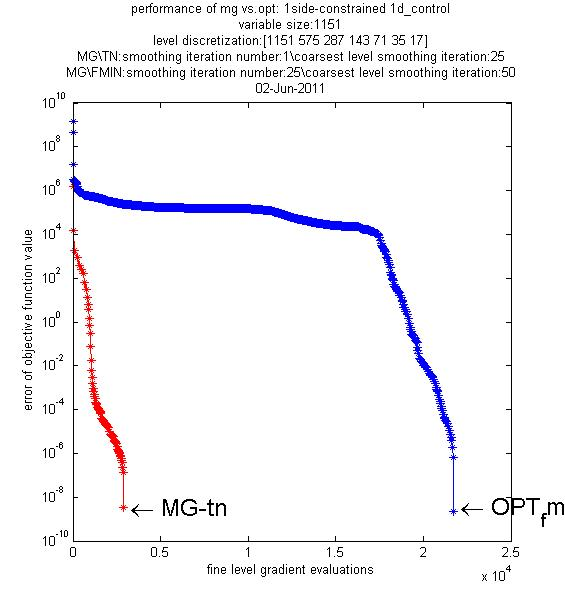
\includegraphics[width=1.0\textwidth]{finalplot11511s.jpg}
  \caption{lower bounds 1-D control problem}
\label{fig:1dcontroll}
\end{figure}

\begin{figure}[h]
\centering
  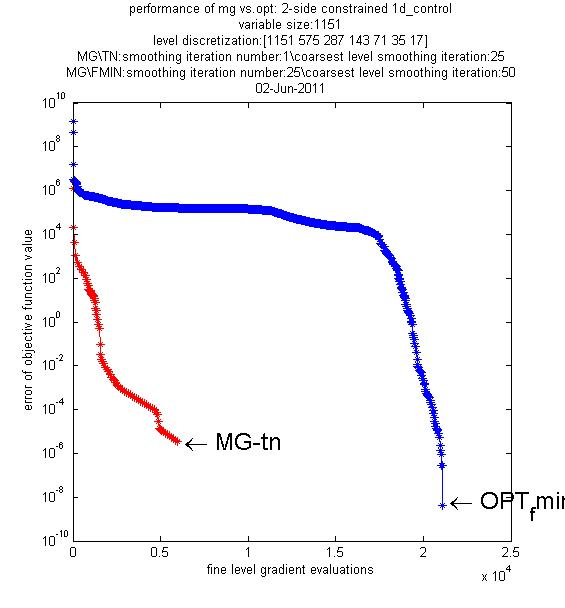
\includegraphics[width=1.0\textwidth]{goodplot11512s.jpg}
  \caption{2-side bounds 1-D control problem}
\label{fig:1dcontrol2}
\end{figure}

\begin{figure}[h]
\centering
  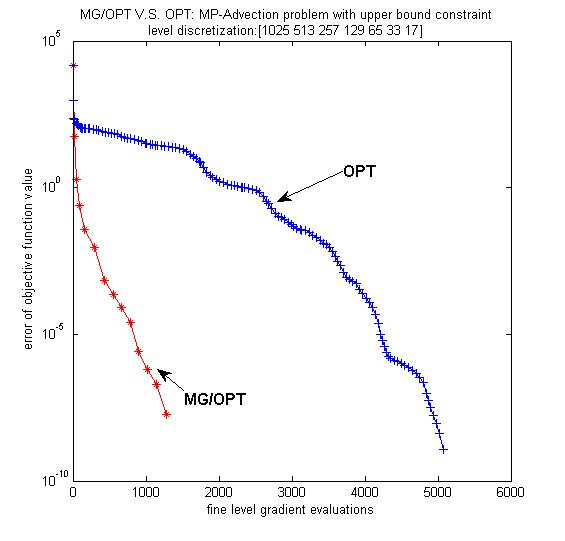
\includegraphics[width=1.0\textwidth]{plot1s1025.jpg}
  \caption{upper bound MG-Advection problem}
\label{fig:advection}
\end{figure}

\begin{figure}[h]
\centering
  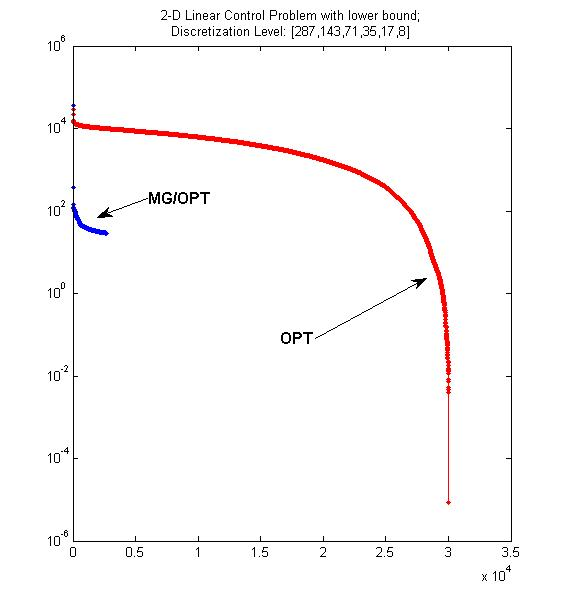
\includegraphics[width=1.0\textwidth]{plot1s287n.jpg}
  \caption{Lower bound  2-D Linear control problem}
\label{fig:bicontrol}
\end{figure}

In figure \ref{fig:1dcontroll}, it demonstrates the performance of MG/OPT comparing to OPT for 1-d control problem with lower bounds.\

In figure \ref{fig:1dcontrol2}, it demonstrates the performance of MG/OPT comparing to OPT for 1-d control problem with both upper and lower bounds.\

In figure \ref{fig:advection}, it demonstrates the performance of MG/OPT comparing to OPT for MP-Advection problem  with upper bounds.The reason MG/OPT didn't reach the same accuracy as OPT did is that the next function value from MG/OPT is smaller than the exact solution I took from OPT.\

In figure \ref{fig:bicontrol}, it demonstrates the performance of MG/OPT comparing to OPT for 2-D Linear control problem  with lower bounds. 
\end{itemize}
\end{document}
